\documentclass[11pt,a4paper]{article}

% ============================================================================
% PAQUETES
% ============================================================================
\usepackage[utf8]{inputenc}
\usepackage[english]{babel}
\usepackage[T1]{fontenc}
\usepackage{amsmath,amssymb,amsfonts}
\usepackage{graphicx}
\usepackage{booktabs}
\usepackage{multirow}
\usepackage{xcolor}
\usepackage{hyperref}
\usepackage{listings}
\usepackage{algorithm}
\usepackage{algpseudocode}
\usepackage{geometry}
\usepackage{fancyhdr}
\usepackage{tikz}
\usetikzlibrary{shapes,arrows,positioning,fit,backgrounds}
\usepackage{subcaption}
\usepackage{float}

\geometry{margin=2.5cm}

% Colores
\definecolor{codegreen}{rgb}{0,0.6,0}
\definecolor{codegray}{rgb}{0.5,0.5,0.5}
\definecolor{codepurple}{rgb}{0.58,0,0.82}
\definecolor{backcolour}{rgb}{0.95,0.95,0.92}
\definecolor{emphblue}{RGB}{41,128,185}
\definecolor{warnred}{RGB}{192,57,43}
\definecolor{successgreen}{RGB}{39,174,96}

% Configuración de listings
\lstdefinestyle{pythonstyle}{
    backgroundcolor=\color{backcolour},
    commentstyle=\color{codegreen},
    keywordstyle=\color{codepurple},
    numberstyle=\tiny\color{codegray},
    stringstyle=\color{emphblue},
    basicstyle=\ttfamily\footnotesize,
    breakatwhitespace=false,
    breaklines=true,
    captionpos=b,
    keepspaces=true,
    numbers=left,
    numbersep=5pt,
    showspaces=false,
    showstringspaces=false,
    showtabs=false,
    tabsize=2,
    language=Python
}
\lstset{style=pythonstyle}

% Headers
\pagestyle{fancy}
\fancyhf{}
\rhead{MS-Predictor: Sistema de Predicción de Brotes}
\lhead{Documentación Técnica}
\rfoot{Página \thepage}

% ============================================================================
% DOCUMENTO
% ============================================================================
\begin{document}

% Título
\begin{titlepage}
    \centering
    \vspace*{2cm}
    
    {\Huge\bfseries MS-Predictor\par}
    \vspace{0.5cm}
    {\Large Sistema de Predicción de Brotes de Esclerosis Múltiple\par}
    \vspace{1cm}
    {\large Mediante Análisis Lingüístico y Machine Learning\par}
    
    \vspace{2cm}
    
    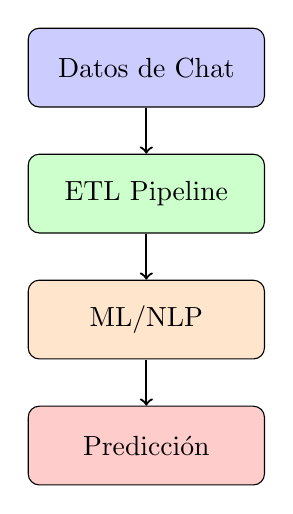
\begin{tikzpicture}[scale=0.8]
        % Diagrama simplificado del sistema
        \node[draw, rounded corners, fill=blue!20, minimum width=3cm, minimum height=1cm] (input) at (0,0) {Datos de Chat};
        \node[draw, rounded corners, fill=green!20, minimum width=3cm, minimum height=1cm] (etl) at (0,-2) {ETL Pipeline};
        \node[draw, rounded corners, fill=orange!20, minimum width=3cm, minimum height=1cm] (ml) at (0,-4) {ML/NLP};
        \node[draw, rounded corners, fill=red!20, minimum width=3cm, minimum height=1cm] (pred) at (0,-6) {Predicción};
        
        \draw[->, thick] (input) -- (etl);
        \draw[->, thick] (etl) -- (ml);
        \draw[->, thick] (ml) -- (pred);
    \end{tikzpicture}
    
    \vfill
    
    {\large\bfseries Documentación Técnica v1.0.0-beta\par}
    \vspace{0.5cm}
    {\large Actualizado: Febrero 2026\par}
    
\end{titlepage}

% Tabla de contenidos
\tableofcontents
\newpage

% ============================================================================
\section{Resumen Ejecutivo}
% ============================================================================

\subsection{Objetivo del Proyecto}

El proyecto \textbf{MS-Predictor} tiene como objetivo desarrollar un sistema de predicción de brotes de Esclerosis Múltiple (EM) con \textbf{7-30 días de antelación}, utilizando:

\begin{itemize}
    \item Análisis lingüístico de comunicaciones (WhatsApp, Telegram)
    \item Patrones de actividad temporal
    \item Features clínicos y de comportamiento
    \item Modelos de Machine Learning y NLP
\end{itemize}

\subsection{Métricas Objetivo y Resultados}

\begin{table}[H]
\centering
\caption{Métricas de Rendimiento del Sistema}
\begin{tabular}{lccc}
\toprule
\textbf{Métrica} & \textbf{Objetivo} & \textbf{Holdout} & \textbf{Walk-Forward} \\
\midrule
AUROC (14 días) & $> 0.65$ & \textcolor{successgreen}{0.6932} & \textcolor{warnred}{0.41 $\pm$ 0.15} \\
AUPRC & $> 0.30$ & 0.3609 & -- \\
Brier Score & $< 0.25$ & TBD & -- \\
\bottomrule
\end{tabular}
\end{table}

\textbf{Hallazgo Crítico:} Existe una discrepancia significativa entre métricas de holdout (0.69) y walk-forward validation (0.41), indicando problemas de generalización temporal que han sido identificados y parcialmente corregidos.

% ============================================================================
\section{Arquitectura del Sistema}
% ============================================================================

\subsection{Visión General}

\begin{figure}[H]
\centering
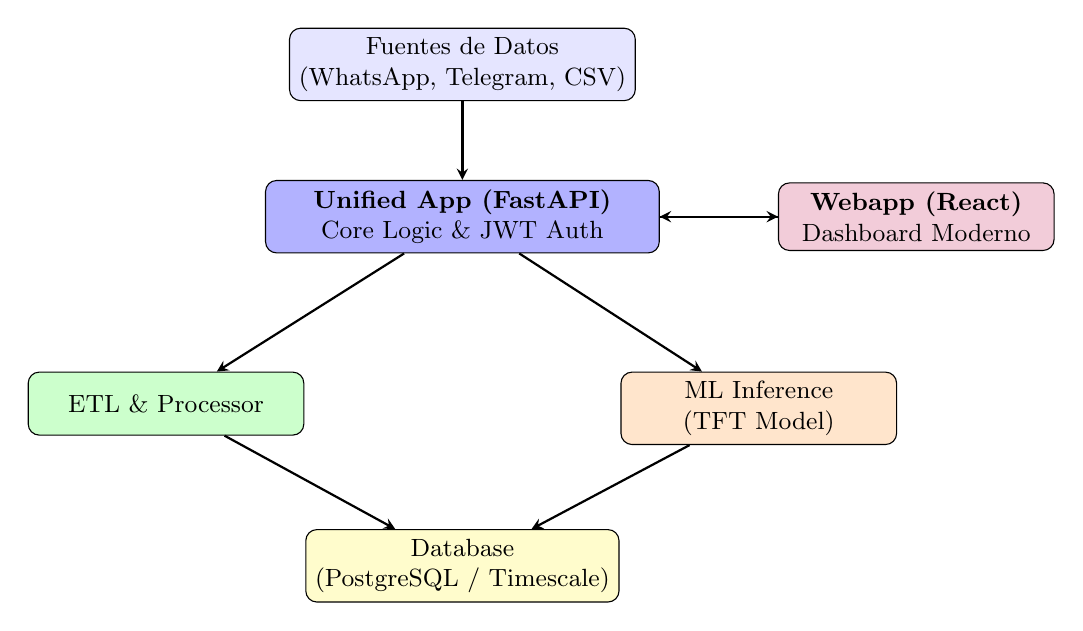
\begin{tikzpicture}[
    node distance=1.5cm,
    block/.style={draw, rounded corners, minimum width=3.5cm, minimum height=0.8cm, align=center, font=\small},
    arrow/.style={->, thick, >=stealth}
]
    % Fuentes de Datos
    \node[block, fill=blue!10] (data) {Fuentes de Datos\\(WhatsApp, Telegram, CSV)};
    
    % Capa de Aplicación
    \node[block, fill=blue!30, below=1cm of data, minimum width=5cm] (unified) {\textbf{Unified App (FastAPI)}\\Core Logic \& JWT Auth};
    
    % Frontend
    \node[block, fill=purple!20, right=1.5cm of unified] (webapp) {\textbf{Webapp (React)}\\Dashboard Moderno};
    
    % Pipeline Interno (Microservicios detrás de la Unified App)
    \node[block, fill=green!20, below left=1.5cm and -0.5cm of unified] (etl) {ETL \& Processor};
    \node[block, fill=orange!20, below right=1.5cm and -0.5cm of unified] (ml) {ML Inference\\(TFT Model)};
    \node[block, fill=yellow!20, below=3.5cm of unified] (db) {Database\\(PostgreSQL / Timescale)};
    
    % Arrows
    \draw[arrow] (data) -- (unified);
    \draw[arrow] (unified) -- (webapp);
    \draw[arrow] (webapp) -- (unified);
    \draw[arrow] (unified) -- (etl);
    \draw[arrow] (unified) -- (ml);
    \draw[arrow] (etl) -- (db);
    \draw[arrow] (ml) -- (db);
    
\end{tikzpicture}
\caption{Arquitectura Evolucionada: Unified Hub Strategy}
\end{figure}

\subsection{Stack Tecnológico}

\begin{table}[H]
\centering
\caption{Stack Tecnológico Actualizado}
\begin{tabular}{lll}
\toprule
\textbf{Componente} & \textbf{Tecnología} & \textbf{Estado} \\
\midrule
Time-series & pytorch-forecasting & Modelo TFT base funcional \\
NLP Backend & SentenceTransformers & Extracción de sentiment y embeddings \\
Database & PostgreSQL + TimescaleDB & Repositorio central de eventos y features \\
\textbf{Unified App} & \textbf{FastAPI} & Orchestrator, JWT, Patient/Doctor Auth \\
\textbf{Frontend} & \textbf{React + Vite + Tailwind} & Dashboard premium v1.0 disponible \\
Deployment & Docker Compose & Stack completo orquestado \\
\bottomrule
\end{tabular}
\end{table}

% ============================================================================
\section{Pipeline de Datos (ETL)}
% ============================================================================

\subsection{Extracción de Datos}

El sistema procesa datos de comunicación de pacientes desde múltiples fuentes:

\begin{lstlisting}[caption={Formatos de entrada soportados}]
FORMATOS_SOPORTADOS = ["whatsapp", "telegram", "csv", "jsonl"]

# Ejemplo de mensaje normalizado
mensaje = {
    "timestamp": "2024-12-01 14:30:00",
    "sender": "paciente",
    "text": "Hoy me siento muy cansada...",
    "metadata": {"source": "whatsapp"}
}
\end{lstlisting}

\subsection{Features Extraídos}

\subsubsection{Features Lingüísticos (por mensaje)}

\begin{itemize}
    \item \textbf{Longitud}: \texttt{char\_count}, \texttt{word\_count}, \texttt{sentence\_count}
    \item \textbf{Diversidad léxica}: \texttt{unique\_words}, \texttt{type\_token\_ratio}
    \item \textbf{Estilo}: \texttt{exclamation\_count}, \texttt{question\_count}, \texttt{caps\_ratio}
    \item \textbf{Expresividad}: \texttt{emoji\_count}
    \item \textbf{Sentiment}: Proxy léxico básico (-1 a +1)
\end{itemize}

\subsubsection{Features Temporales (por día/ventana)}

\begin{itemize}
    \item \textbf{Volumen}: \texttt{messages\_total}, \texttt{messages\_mean}, \texttt{messages\_std}
    \item \textbf{Cobertura}: \texttt{num\_active\_days}, \texttt{coverage}
    \item \textbf{Actividad}: \texttt{active\_hours}, \texttt{night\_ratio}
    \item \textbf{Tendencias}: \texttt{messages\_trend}, \texttt{sentiment\_trend}
\end{itemize}

\subsubsection{Features de Ingeniería}

\begin{lstlisting}[caption={Feature Engineering con prevención de leakage}]
# Lag features (valores de días anteriores)
df[f"{col}_lag{lag}"] = df[col].shift(lag)

# Rolling features CON SHIFT para evitar data leakage
# IMPORTANTE: shift(1) asegura que solo usamos datos hasta t-1
shifted = df[col].shift(1)
df[f"{col}_roll{window}_mean"] = shifted.rolling(window).mean()
df[f"{col}_roll{window}_std"] = shifted.rolling(window).std()
df[f"{col}_roll{window}_trend"] = shifted.rolling(window).apply(
    lambda x: np.polyfit(range(len(x)), x, 1)[0]
)
\end{lstlisting}

\subsection{Generación de Labels}

\begin{equation}
y_{t,h} = \begin{cases}
1 & \text{si existe evento en } [t+1, t+h] \\
0 & \text{en caso contrario}
\end{cases}
\end{equation}

Donde $h \in \{7, 14, 30\}$ días son los horizontes de predicción.

% ============================================================================
\section{Modelos de Machine Learning}
% ============================================================================

\subsection{Modelos Baseline}

\subsubsection{Random Forest}

Configuración optimizada mediante Optuna:

\begin{lstlisting}
RandomForestClassifier(
    n_estimators=58,
    max_depth=13,
    min_samples_split=8,
    min_samples_leaf=4,
    class_weight="balanced"
)
\end{lstlisting}

\subsubsection{Gradient Boosting Machine (GBM)}

\begin{lstlisting}
GradientBoostingClassifier(
    n_estimators=89,
    max_depth=6,
    learning_rate=0.018,
    min_samples_split=7,
    subsample=0.92
)
\end{lstlisting}

\subsection{Temporal Fusion Transformer (TFT)}

El modelo principal de producción utiliza la arquitectura \textit{Temporal Fusion Transformer}, diseñada específicamente para series temporales multivariantes con horizontes múltiples.

\begin{itemize}
    \item \textbf{Encoder length}: 30 días de historia lingüística y de actividad.
    \item \textbf{Prediction length}: 14 días (horizonte objetivo).
    \item \textbf{Loss function}: \textit{Quantile Loss} para capturar la incertidumbre en la predicción del riesgo.
    \item \textbf{Features dinámicos}: Sentiment mean/std, activity coverage, messages trend, response latency.
\end{itemize}

\begin{lstlisting}[caption={Configuración del dataset TFT}]
training = TimeSeriesDataSet(
    df,
    target=target_col,
    group_ids=['user_id_hash'],
    max_encoder_length=30,
    max_prediction_length=14,
    time_varying_unknown_reals=[
        'sentiment_mean', 'sentiment_trend',
        'num_messages_total', 'response_latency_mean',
        'steps_mean', 'sleep_hours_mean'
    ],
    target_normalizer=GroupNormalizer(groups=['user_id_hash']),
)
\end{lstlisting}

\subsection{Ensemble Methods}

\begin{table}[H]
\centering
\caption{Comparación de Métodos Ensemble}
\begin{tabular}{lcc}
\toprule
\textbf{Método} & \textbf{AUROC} & \textbf{AUPRC} \\
\midrule
Random Forest & 0.5917 & 0.3032 \\
\textbf{GBM} & \textbf{0.6932} & \textbf{0.3609} \\
Logistic Regression & 0.1623 & 0.1635 \\
Voting (Soft) & 0.5928 & 0.3044 \\
Stacking & 0.4578 & 0.2416 \\
Manual Average & 0.6511 & 0.3282 \\
\bottomrule
\end{tabular}
\end{table}

\subsection{Validación Temporal}

\subsubsection{Walk-Forward Validation con Embargo}

Para evaluar correctamente modelos de series temporales, implementamos validación walk-forward con:

\begin{itemize}
    \item \textbf{Gap (embargo)}: Período entre fin de train y inicio de test
    \item \textbf{Purge}: Eliminación de últimos N días del train (sus labels miran al futuro)
\end{itemize}

\begin{algorithm}[H]
\caption{Walk-Forward Validation con Embargo}
\begin{algorithmic}[1]
\Require Dataset $D$, train\_window, test\_window, gap, purge
\State Ordenar $D$ por fecha
\State $t \gets 0$
\While{$t + \text{train\_window} + \text{gap} + \text{test\_window} \leq |D|$}
    \State $\text{train\_end} \gets t + \text{train\_window} - \text{purge}$
    \State $\text{test\_start} \gets t + \text{train\_window} + \text{gap}$
    \State $\text{test\_end} \gets \text{test\_start} + \text{test\_window}$
    \State $D_{\text{train}} \gets D[t : \text{train\_end}]$
    \State $D_{\text{test}} \gets D[\text{test\_start} : \text{test\_end}]$
    \State Entrenar modelo en $D_{\text{train}}$
    \State Evaluar en $D_{\text{test}}$
    \State $t \gets t + \text{step}$
\EndWhile
\end{algorithmic}
\end{algorithm}

% ============================================================================
\section{Análisis de Data Leakage}
% ============================================================================

\subsection{Problema Identificado}

Se detectó una discrepancia significativa entre métricas:

\begin{equation}
\text{AUROC}_{\text{holdout}} - \text{AUROC}_{\text{walk-forward}} = 0.69 - 0.41 = 0.28
\end{equation}

\subsection{Fuentes de Leakage}

\begin{enumerate}
    \item \textbf{Rolling Features sin Shift}: Los features de ventana móvil incluían datos del día actual ($t=0$).
    
    \item \textbf{Validación sin Gap}: El test comenzaba inmediatamente después del train, pero el target \texttt{relapse\_in\_14d} mira 14 días hacia adelante.
    
    \item \textbf{Labels Contaminados}: Los últimos 14 días del train tienen labels que dependen del período de test.
\end{enumerate}

\subsection{Correcciones Implementadas}

\begin{table}[H]
\centering
\caption{Correcciones de Data Leakage}
\begin{tabular}{lp{8cm}}
\toprule
\textbf{Corrección} & \textbf{Implementación} \\
\midrule
Shift en rolling & \texttt{df[col].shift(1).rolling(window).mean()} \\
Gap temporal & Parámetro \texttt{--gap 14} en walk-forward \\
Purge de train & Parámetro \texttt{--purge 14} para eliminar últimos días \\
Auditoría & Script \texttt{validate\_no\_leakage.py} \\
\bottomrule
\end{tabular}
\end{table}

% ============================================================================
\section{NLP y Embeddings de Texto}
% ============================================================================

\subsection{Sentence Transformers (Baseline)}

El sistema utiliza \texttt{SentenceTransformer} para generar embeddings de 384 o 768 dimensiones que capturan el contexto semántico de las comunicaciones diarias.

\begin{itemize}
    \item \textbf{Modelo}: \texttt{multilingual-e5-large} o \texttt{paraphrase-multilingual-MiniLM-L12-v2}.
    \item \textbf{Pooling}: Mean pooling sobre los tokens de la ventana diaria.
\end{itemize}

\subsection{MiniLLM v2: Análisis de Perplexity}

Como innovación técnica, se integra \textbf{MiniLLM v2 (TinyGPTv2)}, un modelo de lenguaje especializado que permite extraer métricas de la dinámica lingüística del paciente.

\begin{itemize}
    \item \textbf{Perplexity}: Mide la "sorpresa" del modelo ante el texto del paciente. Aumentos en perplexity pueden indicar desorientación cognitiva o fatiga prodrómica.
    \item \textbf{Attention Entropy}: Mide la dispersión del foco de atención en el texto generado.
\end{itemize}

\begin{lstlisting}[caption={Extracción de Perplexity con MiniLLM}]
def compute_perplexity(self, text: str) -> float:
    tokens = self.tokenizer.encode(text).ids
    logits, _ = self.model(torch.tensor([tokens]))
    
    shift_logits = logits[:, :-1, :].contiguous()
    shift_labels = tokens_tensor[:, 1:].contiguous()
    
    loss = functional.cross_entropy(
        shift_logits.view(-1, shift_logits.size(-1)),
        shift_labels.view(-1),
    )
    return torch.exp(loss).item()
\end{lstlisting}

% ============================================================================
\section{Propuestas de Mejora}
% ============================================================================

\section{Hoja de Ruta y Próximos Pasos}

\subsection{Corto Plazo: Refinamiento del Modelo}

\begin{enumerate}
    \item \textbf{Calibración de Probabilidades}: Implementar \textit{Platt Scaling} para que las probabilidades de riesgo sean más precisas clínicamente.
    
    \item \textbf{Feature Selection Dinámico}: Utilizar las métricas de atención del TFT para descartar features lingüísticos irrelevantes.
    
    \item \textbf{Optimización de Latencia}: Reducir el tiempo de inferencia del \texttt{nlp-agent} mediante cuantización (int8) de los Sentence Transformers.
\end{enumerate}

\subsection{Medio Plazo: Expansión de Capacidad}

\begin{enumerate}
    \item \textbf{Multi-persona Validation}: Entrenar el modelo con datos agregados de múltiples pacientes para mejorar la generalización (Cross-patient validation).
    
    \item \textbf{Integración MiniLLM Local}: Sustituir APIs externas por un modelo \textit{TinyLlama} local para análisis de perplexity en tiempo real sin salir del servidor.
\end{enumerate}

\subsection{Largo Plazo: Hacia la Certificación}

\begin{enumerate}
    \item \textbf{Validación Clínica Rigurosa}: Estudio piloto con un grupo de control para medir la reducción de falsos positivos en la detección de brotes.
    
    \item \textbf{Privacidad Diferencial}: Implementar mecanismos de ruidos estadísticos para permitir el entrenamiento federado sin comprometer datos individuales.
\end{enumerate}

% ============================================================================
\section{Pipeline de Inferencia Implementado}
% ============================================================================

\begin{figure}[H]
\centering
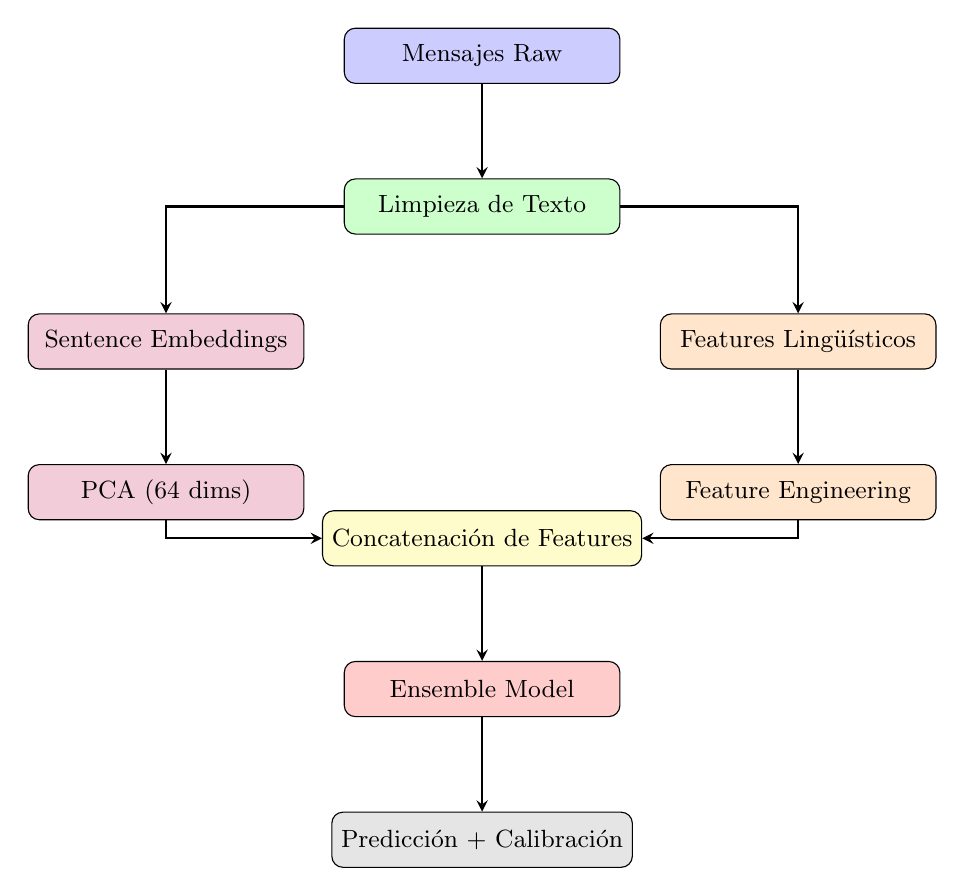
\begin{tikzpicture}[
    node distance=1.2cm,
    block/.style={draw, rounded corners, minimum width=3.5cm, minimum height=0.7cm, align=center, font=\small},
    arrow/.style={->, thick, >=stealth}
]
    % Input
    \node[block, fill=blue!20] (raw) {Mensajes Raw};
    
    % Preprocesamiento
    \node[block, fill=green!20, below=of raw] (clean) {Limpieza de Texto};
    
    % Rama NLP
    \node[block, fill=purple!20, below left=1cm and 0.5cm of clean] (embed) {Sentence Embeddings};
    \node[block, fill=purple!20, below=of embed] (pca) {PCA (64 dims)};
    
    % Rama Features tradicionales
    \node[block, fill=orange!20, below right=1cm and 0.5cm of clean] (feat) {Features Lingüísticos};
    \node[block, fill=orange!20, below=of feat] (eng) {Feature Engineering};
    
    % Fusión
    \node[block, fill=yellow!20, below=1.5cm of clean, yshift=-2cm] (fusion) {Concatenación de Features};
    
    % Modelo
    \node[block, fill=red!20, below=of fusion] (model) {Ensemble Model};
    
    % Output
    \node[block, fill=gray!20, below=of model] (pred) {Predicción + Calibración};
    
    % Arrows
    \draw[arrow] (raw) -- (clean);
    \draw[arrow] (clean) -| (embed);
    \draw[arrow] (clean) -| (feat);
    \draw[arrow] (embed) -- (pca);
    \draw[arrow] (feat) -- (eng);
    \draw[arrow] (pca) |- (fusion);
    \draw[arrow] (eng) |- (fusion);
    \draw[arrow] (fusion) -- (model);
    \draw[arrow] (model) -- (pred);
    
\end{tikzpicture}
\caption{Pipeline Propuesto con Integración de NLP}
\end{figure}

% ============================================================================
\section{Conclusiones}
% ============================================================================

\subsection{Estado Actual}

\begin{itemize}
    \item \textbf{Infraestructura Unificada}: Se ha consolidado el backend en una \textit{Unified App} que gestiona seguridad, datos y orquestación.
    \item \textbf{Interfaz Clínica}: El nuevo dashboard en React permite la visualización de riesgos, gestión de eventos clínicos y monitoreo de servicios.
    \item \textbf{Pipeline de Eventos}: Implementada la capacidad de registrar brotes, cambios de medicación y otros eventos clínicos directamente desde la UI.
\end{itemize}

\subsection{Limitaciones y Desafíos}

\begin{itemize}
    \item \textbf{Generalización}: Aún persiste la brecha entre validación holdout y walk-forward.
    \item \textbf{Volumen de Datos}: Se requiere la incorporación de más sujetos para mejorar la robustez del modelo TFT.
\end{itemize}

\subsection{Pasos Siguientes Priorizados}

\begin{enumerate}
    \item \textbf{Validación Clínica E2E}: Iniciar pruebas selectas con facultativos utilizando el nuevo dashboard.
    \item \textbf{Refubish de NLP}: Sustituir el proxy básico de sentiment por el motor \texttt{nlp-agent} completo.
    \item \textbf{Inferencia en Tiempo Real}: Optimizar la latencia del proxy de predicción en la Unified App.
\end{enumerate}

% ============================================================================
% APÉNDICES
% ============================================================================
\appendix

\section{Estructura de Archivos del Proyecto}

\begin{lstlisting}[language=bash, caption={Estructura actual de servicios}]
PreSickness/
├── services/
│   ├── unified_app/     # Core API & Orchestration
│   ├── webapp/          # Frontend React/Vite
│   ├── ml-inference/    # Motor de prediccion TFT
│   ├── nlp-agent/       # Analisis lingüistico avanzado
│   ├── feature-extractor/ # Procesamiento de ventanas
│   └── alert-manager/   # Gestion de notificaciones
├── scripts/
│   ├── etl/             # Pipelines de datos
│   └── ml/              # Entrenamiento y validacion
├── data/                # Datasets procesados
├── docs/                # Documentación técnica
└── docker-compose.yml   # Orquestación de infraestructura
\end{lstlisting}

\section{Comandos de Ejecución}

\begin{lstlisting}[language=bash, caption={Comandos principales}]
# ETL
python -m scripts.etl.pipeline \
    --input datos/paciente1_whatsapp.txt \
    --events datos/paciente1_events.csv \
    --patient-id paciente1

# Feature Engineering
python scripts/ml/feature_engineering.py \
    --data-path data/processed/paciente1

# Optimizacion de Hiperparametros
python scripts/ml/optuna_simple.py \
    --data-path data/processed/paciente1 \
    --n-trials 30

# Validacion Walk-Forward con Embargo
python scripts/ml/walk_forward_validation.py \
    --data-path data/processed/paciente1 \
    --gap 14 \
    --purge 14

# Auditoria de Data Leakage
python scripts/ml/validate_no_leakage.py \
    --data-path data/processed/paciente1
\end{lstlisting}

% ============================================================================
\end{document}
